\documentclass[12pt]{article}%
\usepackage{amsfonts}
\usepackage{fancyhdr}
\usepackage{comment}
\usepackage[a4paper, top=2.5cm, bottom=2.5cm, left=2.2cm, right=2.2cm]%
{geometry}
\usepackage{times}
\usepackage{amsmath}
\usepackage{changepage}
\usepackage{stfloats}
\usepackage{amssymb}
\usepackage{graphicx}
\usepackage{indentfirst}

\setlength{\parindent}{2em}
\setcounter{MaxMatrixCols}{30}
\newtheorem{theorem}{Theorem}
\newtheorem{acknowledgement}[theorem]{Acknowledgement}
\newtheorem{algorithm}[theorem]{Algorithm}
\newtheorem{axiom}{Axiom}
\newtheorem{case}[theorem]{Case}
\newtheorem{claim}[theorem]{Claim}
\newtheorem{conclusion}[theorem]{Conclusion}
\newtheorem{condition}[theorem]{Condition}
\newtheorem{conjecture}[theorem]{Conjecture}
\newtheorem{corollary}[theorem]{Corollary}
\newtheorem{criterion}[theorem]{Criterion}
\newtheorem{definition}[theorem]{Definition}
\newtheorem{example}[theorem]{Example}
\newtheorem{exercise}[theorem]{Exercise}
\newtheorem{lemma}[theorem]{Lemma}
\newtheorem{notation}[theorem]{Notation}
\newtheorem{problem}[theorem]{Problem}
\newtheorem{proposition}[theorem]{Proposition}
\newtheorem{remark}[theorem]{Remark}
\newtheorem{solution}[theorem]{Solution}
\newtheorem{summary}[theorem]{Summary}
\newenvironment{proof}[1][Proof]{\textbf{#1.} }{\ \rule{0.5em}{0.5em}}

\usepackage{mathtools}

\newcommand{\Q}{\mathbb{Q}}
\newcommand{\R}{\mathbb{R}}
\newcommand{\C}{\mathbb{C}}
\newcommand{\Z}{\mathbb{Z}}

\begin{document}

\title{MATH2040C Homework 7}
\author{ZHENG Weijia (William, 1155124322)}
\date{April 25, 2021}
\maketitle

\large

\section{Section 6.3, Q3(c)}

\begin{figure}[htp]
    \centering % 图片居中
    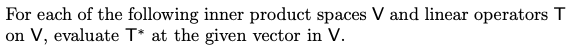
\includegraphics[width = 16cm]{img/Q1a.png}
    \includegraphics*[width = 15cm]{img/Q1b.png}
    %\caption{Section 6.1 Q8}
    %\label{fig:figure1label}
\end{figure}


The first thing we need to do is to find a orthonormal basis for $V$.

A basis for $V$ is $\alpha=\{1,t\}.$ Note that $\int_{-1}^{1}1\cdot t ~dt =0.$
Therefore $\alpha$ is an orthogonal basis. Applying the Gram-Schmidt process, we can 
generate an orthonormal basis $\beta=\{\frac{1}{\sqrt{2}},\frac{\sqrt{3}t}{\sqrt{2}} \}$.

Then according to Remark 16.3, we can have 
$$T^* (g(t))=\sum_{i=1}^n \overline{\langle T(v_i),g(t) \rangle} v_i.$$

With $T(\frac{1}{\sqrt{2}})=\frac{3}{\sqrt{2}}$. 
And $T(\sqrt{\frac{3}{2}}t)=\sqrt{\frac{3}{2}}+3\sqrt{\frac{3}{2}}t.$. 

Therefore, $$T^*(g(t))=\frac{3}{2}\int_{-1}^1 g(t)dt + \frac{3}{2}t\int_{-1}^1 (1+3t)g(t)dt.$$

The given vector is $f(t)=4-2t.$ Hence the answer should be 
$$T^*(4-2t)=12+6t.$$

Done.



\newpage

\section{Section 6.3, Q13}

\begin{figure}[htp]
    \centering % 图片居中
    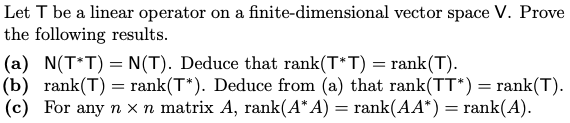
\includegraphics[width = 16cm]{img/Q2.png}
    %\caption{Section 6.1 Q8}
    %\label{fig:figure1label}
\end{figure}

\subsection{(a)}
Note that $\forall x \in N(T),$ $$T^*Tx = T^*(Tx)=T^*(0)=0.$$

Therefore $x\in N(T^*T).$ Hence $N(T) \subset N(T^*T).$

Forall $y \in N(T^*T), $ consider the norm of $Ty:$ 
$$||Ty||^2=\langle Ty,Ty \rangle=\langle y, T^*Ty \rangle = \langle y,0 \rangle=0.$$

Which implies that $Ty=0.$ Therefore $y \in N(T).$ Hence $N(T^*T) \subset N(T).$

Based on all above, $N(T^*T)=N(T).$

Recall that $T \in \mathcal{L}(V).$ Hence $T:V \to V.$ And according to $\forall y \in V,$
$$T^*(y)=\sum_{i=1}^n \overline{\langle T(v_i),y \rangle} v_i.$$

We know that $T^*:V \to V.$ Therefore $T^*T:V \to V.$

Applying the rank nullity theorem, we have that 
$$\dim{V} = rank(T^*T)+\dim{N(T^*T)}~,~\dim{V} = rank(T)+\dim{N(T)}.$$

Using the just proved fact $N(T^*T)=N(T),$ we can simply deduce $$rank(T^*T)=rank(T).$$

\subsection{(b)}
By changing name of the identity in (a), we can have $N(TT^*)=N(T^*)$ and $rank(TT^*)=rank(T^*).$

Notice that $$rank(T)=rank[T]_\beta=rank[T]_\beta^*=rank[T^*]_\beta=rank(T^*).$$

And then $rank(TT^*)=rank(T)$ follows.

\subsection{(c)}
From (b), $rank(AA^*)=rank(A)$ follows naturally. 

And note that $(AA^*)^* =A^*A$, then $$rank(AA^*)=rank(A^*A).$$

Therefore, $$rank(AA^*)=rank(A^*A)=rank(A).$$

Done.


\noindent\rule[0.1ex]{\linewidth}{1pt}


\section{Section 6.3, Q14}
\begin{figure}[htp]
    \centering % 图片居中
    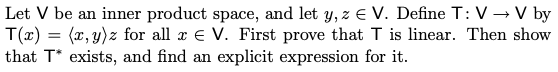
\includegraphics[width = 16cm]{img/Q3.png}
    %\caption{Section 6.1 Q8}
    %\label{fig:figure1label}
\end{figure}

First we would prove that $T$ is linear. $\forall x_1,x_2 \in V, \forall c \in F,$
$$T(cx_1+x_2)=\langle cx_1+x_2,y \rangle z = \langle cx_1,y \rangle z + \langle x_2,y \rangle z=c\langle x_1,y \rangle z+\langle x_2,y \rangle z.$$

The equalities are deduced from the properties of inner product. And hence $$T(cx_1+x_2)=cT(x_1)+T(x_2).$$

Therefore, $T$ is linear. 

From course not we directly construct $\forall x \in V,$ 
$$T^*(x)=\sum_{i=1}^n\ \overline{\langle T(v_i),x \rangle}v_i
=\sum_{i=1}^n \overline{ \langle \langle v_i,y \rangle z, x \rangle }v_i
=\overline{\langle z,x \rangle} \sum_{i=1}^n \overline{\langle v_i,y \rangle} v_i=\overline{\langle z,x \rangle}y.$$

Recall that $y=I(y)=I^*(y)=\sum_{i=1}^n\ \overline{\langle I(v_i),y \rangle}v_i=\sum_{i=1}^n\ \overline{\langle v_i,y \rangle}v_i.$ Hence the last 
equality holds properly.


\newpage

\section{Section 6.3, Q15}
\begin{figure}[htp]
    \centering % 图片居中
    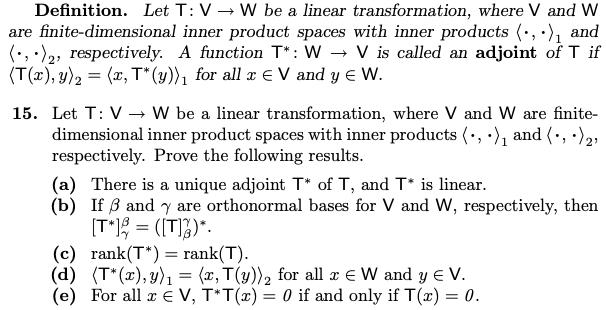
\includegraphics[width = 17cm]{img/Q4.png}
    %\caption{Section 6.1 Q8}
    %\label{fig:figure1label}
\end{figure}

\subsection{(a)}
Define $g:V \to F$ by $g(x)=\langle T(x),y \rangle_2.$ Obviously, note that
$g$ is linear for sure.

Then apply the theorem 6.8, there exists a unique vector $y' \in W$ such that 
$$g(x)=\langle x,y' \rangle_1.$$

Recall $g$'s definition, we have $\langle T(x),y \rangle_2=\langle x,y' \rangle_1, ~\forall x \in V.$

Define that $T^*:W \to V$ by $T^*(y)=y'.$

Then we have $\langle T(x),y \rangle_2=\langle x,T^*(y) \rangle_1.$

Hence the wanted $T^*$ function exists, and becasue the $y'$ is "unique" as mentioned above (for any y),
then the $T^*$ is also unique.

~\ 


Then we prove the linearity of $T^*.$ $\forall y_1,y_2 \in W$ and $\forall c \in F$,
$$\langle x,T^*(cy_1+y_2) \rangle_1 = \langle T(x),cy_1+y_2 \rangle_2
=\langle x, cT^*(y_1) \rangle_1 + \langle x, T^*(y_2) \rangle_1 $$
$$=\langle x, cT^*(y_1)+T^*(y_2) \rangle_1, \forall x \in V.$$

Therefore $T^*(cy_1+y_2) = cT^*(y_1)+T^*(y_2).$ Hence $T^*$ is linear.

\subsection{(b)}
For such kind of problem, we need to compare the two matrices entry wise.
Denote $\beta=\{v_1,v_2,\dots, v_n\}, \gamma=\{w_1,w_2,\dots,w_m\}.$

Inspect $[T^*]_\gamma^{\beta}=[T^*(w_1),T^*(w_2),\dots,T^*(w_m)]_\beta.$

Note that $T^*(w_j)=\sum_{i=1}^n \overline{\langle v_i,T^*(w_j) \rangle_1}v_i, ~\forall j=1,2,\dots,m.$

From this we know that the i-th row, j-th column of $[T^*]_\gamma^{\beta}$ is $\overline{\langle v_i,T^*(w_j) \rangle_1}.$

Inspect $[T]_\beta^{\gamma}=[T(v_1),T(v_2),\dots,T(v_n)]_\gamma$.

Note that $T(v_i)=\sum_{k=1}^m \overline{\langle w_k,T(v_i) \rangle_2}w_k, ~\forall i=1,2,\dots,n.$

Therefore, the i-th column, k-th row of $[T]_{\beta}^{\gamma}=\overline{\langle w_k,T(v_i) \rangle_2}.$

Hence, for $([T]_{\beta}^{\gamma})^*$, the i-th row, j-th column is $\langle w_j,T(v_i) \rangle_2$.

What remains to be done is to show $$\langle w_j,T(v_i) \rangle_2 = \overline{\langle v_i,T^*(w_j) \rangle_1}.$$

This is equivalent to show $\overline{\langle w_j,T(v_i) \rangle_2} = \langle v_i,T^*(w_j) \rangle_1.$

Note that the L.H.S.=$\langle T(v_i),w_j \rangle_2$=R.H.S. from the definition of $T^*.$ Hence this is proved.

\subsection{(c)}

$rank(T^*)=rank([T^*]_\gamma^{\beta})$ and $rank(T)=rank([T]_\beta^{\gamma})=rank(([T]_\beta^{\gamma})^*).$

Followed from (b), we have $rank(T^*)=rank(T).$

\subsection{(d)}
We want to prove $\langle T^*(y),x \rangle_1=\langle y,T(x) \rangle_2, \forall y\in W, x \in V.$ 
which is equivalent to prove $\langle x, T^*(y) \rangle_1=\langle T(x),y \rangle_2$.

And L.H.S.=$\langle T(x),y \rangle_2$ followed from the definition of $T^*$.

Done.

\subsection{(e)}
It is suffice to prove $N(T)=N(T^*T).$ And it is obvious to see that $$N(T) \subset N(T^*T).$$

Take any $x$ such that $T^*Tx = 0.$ We have $\langle Tx,Tx \rangle_2=\langle x,T^*Tx \rangle_1=0.$ 
Which implies that $Tx=0.$ Hence $x \in N(T),$ and $N(T^*T)=N(T).$

Done.

\newpage

\section{Section 6.4, Q2(d)}
\begin{figure}[htp]
    % \centering % 图片居中
    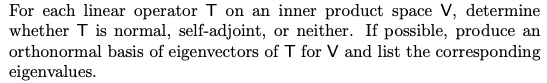
\includegraphics[width = 16cm]{img/Q5a.png}
    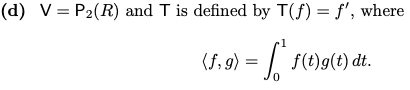
\includegraphics[width = 10cm]{img/Q5b.png}
    %\caption{Section 6.1 Q8}
    %\label{fig:figure1label}
\end{figure}

Let $\{1,t,t^2\}$ be a basis for $P_2(\mathbb{R})$, then apply Gram-Schmidt process upon it, 
we can have an orthonormal basis $\beta=\{1,2\sqrt{3}(t-\frac{1}{2}),6\sqrt{5}(t^2-t+\frac{1}{6})\}.$

First, we claim that $T$ is not self-adjoint, by the spectral theorem, $T$ is 
self-adjoint iff, $T$ is diagnoalizable, which implies that it will lead to the 
eigenspace decomposition of $V$. Note that there is only one eigenvalue of $T$, 
which is 0 and the only corresponding set 
of eigenvectors is $span\{1\}$. It is obvious that $E_0 \neq V,$ 
since $t^2 \notin E_0.$ Therefore $T$ is not self-adjoint and meanwhile, 
it is impossible to derive a orthonormal basis of eigenvectors of T for V.

Also, $T$ is not normal.


\newpage

\section{Section 6.4, Q7}
\begin{figure}[htp]
    \centering % 图片居中
    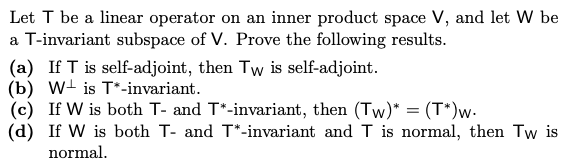
\includegraphics[width = 16cm]{img/Q6.png}
    %\caption{Section 6.1 Q8}
    %\label{fig:figure1label}
\end{figure}

\subsection{(a)}
Denote $\dim{V}=n,\dim{W}=m$, with $m\leq n.$ Let $\beta=\{v_1,v_2,\dots,v_n\}$
be an orthonormal basis for $V$, $\beta_W=\{v_1,v_2,\dots,v_m\}$ be an orthonormal basis for $W$.

$\forall y\in W,$ $T_W(y)=T(y)=\sum_{i=1}^n \langle T(y),v_i \rangle v_i=T^*(y).$ Because $T$ is a self adjoint opeartor.

From the construction rule of adjoint, we have 
$T^*(y)=\sum_{i=1}^n \overline{\langle T(v_i),y \rangle} v_i.$

From the question, we know that $W$ is T-invarian, then $T_W(y) \in W.$ Combined with $v_i$'s are 
linear independent, then 
$$T_W(y)=\sum_{i=1}^m \overline{\langle T(v_i),y \rangle} v_i=\sum_{i=1}^m \overline{\langle T_W(v_i),y \rangle} v_i.$$

Note that the R.H.S. is the definition of $T_W^*(y).$ Hence $$T_W(y)=T_W^*(y), \forall y \in W.$$

\subsection{(b)}
















\end{document}